\documentclass{birkjour}
\usepackage{graphicx,amsopn,amsthm,amsfonts}
\DeclareMathOperator{\area}{area}
\DeclareMathOperator{\comp}{comp}

\setlength{\parskip}{1.3ex plus0.3ex minus0.3ex}
\setlength{\parindent}{0em}

\input{pat}

\listfiles
%Geombinatorics formatting...
%\setlength{\oddsidemargin}{0.35in}
%\setlength{\evensidemargin}{0.35in}
%\setlength{\topmargin}{0.35in}
%\setlength{\headheight}{0in}
%\setlength{\headsep}{0in}
%\setlength{\topskip}{0in}
%\setlength{\footskip}{0in}
%\setlength{\textwidth}{4.8in}
%\setlength{\textheight}{7.65in}
%\pagestyle{empty}

\begin{document}

\title[A Generalized Winternitz Theorem]{A Generalized Winternitz Theorem}

\author{Prosenjit Bose}
\address{School of Computer Science \\ Carleton University \\ 1125 Colonel By Drive \\ Ottawa CANADA K1S 5B6}
\email{jit@scs.carleton.ca}

\author{Paz Carmi}
\address{
Department of Computer Science  \\
Ben-Gurion University of the Negev \\
Beer-Sheva 84105, Israel}
\email{carmip@cs.bgu.ac.il}

\author{Ferran Hurtado}
\address{
Departament de Matem\`atica Aplicada II  \\
Universitat Polit\`ecnica de Catalunya (UPC)   \\
Edifici Omega, Campus Nord  \\
Jordi Girona, 1-3 \\                                           
E-08034 Barcelona  \\  
Spain}
\email{Ferran.Hurtado@upc.edu}

\author{Pat Morin}
\address{School of Computer Science \\ Carleton University \\ 1125 Colonel By Drive \\ Ottawa CANADA K1S 5B6}
\email{morin@scs.carleton.ca}

\subjclass{51E99}
\keywords{Winternitz' Theorem, Centerpoint Theorem, Polygons}
\date{\today}

\begin{abstract}
We prove that, for every simple polygon $P$ having $k\ge 1$ reflex
vertices, there exists a point $q\in P$ such that every half-polygon
that contains $q$ contains nearly $1/2(k+1)$ times the area of $P$.
We also give a family of examples showing that this result is the best
possible.
\end{abstract}


%\begin{center}
%  \textbf{A Generalized Winternitz Theorem} \\
%  Prosenjit Bose, Paz Carmi, Ferran Hurtado, and Pat Morin 
%\end{center}
%\begin{center}
%  School of Computer Science \\ 
%  Carleton University \\
%  \{jit,paz,morin\}@cg.scs.carleton.ca
%\end{center}
%\begin{center}
%  Departament de Matem\`atica Aplicada II \\
%  Universitat Polit\`ecnica de Catalunya \\
%  Ferran.Hurtado@upc.edu
%\end{center}
\maketitle


\section{Introduction}
\emph{Winternitz' Theorem} \cite[pp.~54--55]{b23} is a classic theorem
in convex geometry that has been rediscovered many times
\cite{e55b,ll35,n45,n58,yb51}.  Winternitz' Theorem states that, for
any convex polygon $P$, there exists a point $q\in P$ such that any
halfspace that contains $q$ contains at least $4/9$ of the area of
$P$.  The dissection of a triangle into 9 similar triangles shown in
\figref{winternitz} can easily be used to show that the bound of $4/9$
is tight when $P$ is a triangle.
\let\thefootnote\relax\footnote{Prosenjit Bose and Pat Morin funded by NSERC. Ferran Hurtado funded by projects MTM2009-07242 and 2009SGR1040. Paz Carmi funded by a grant from the German-Israeli Science Foundation.  }

\begin{figure}[htbp]
  \begin{center}
    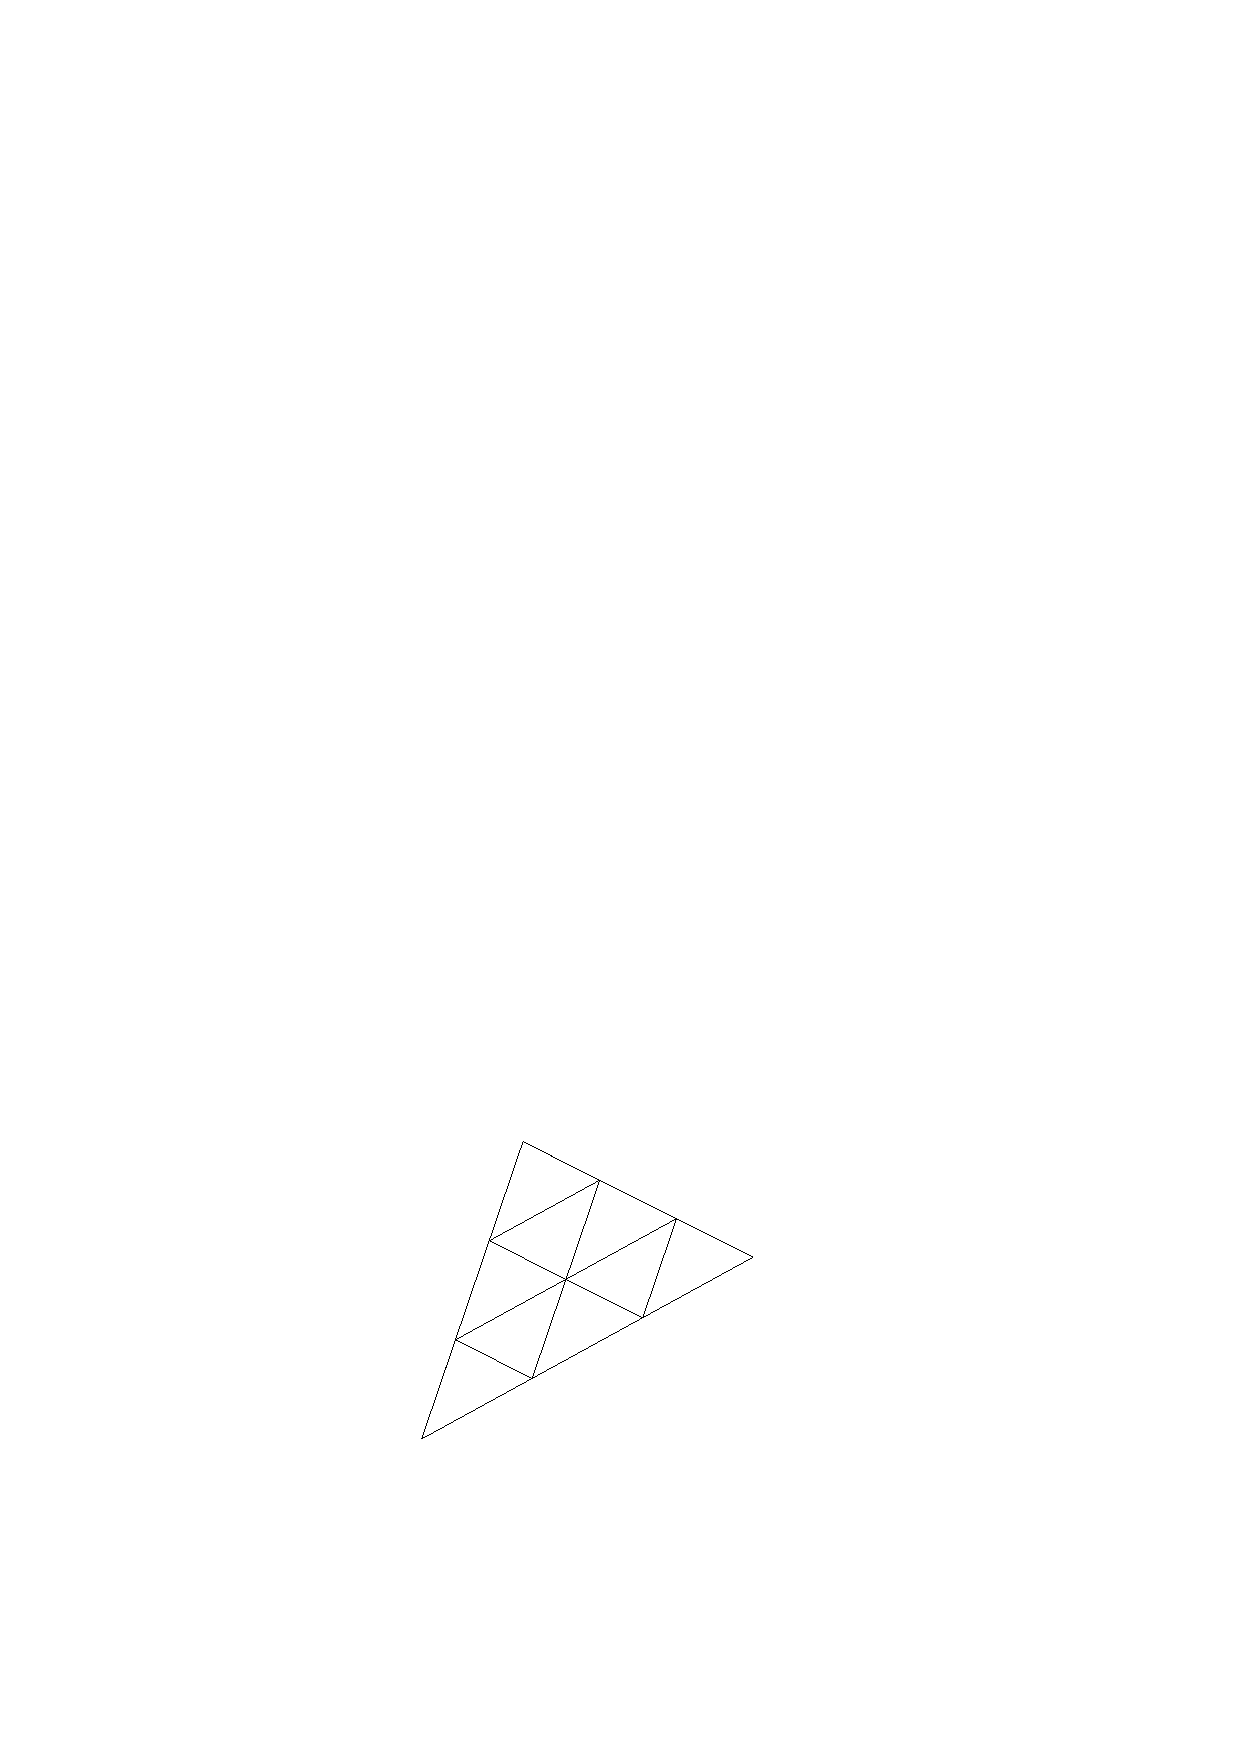
\includegraphics{2089-figure1}
  \end{center}
  \caption{A triangle has maximum halfspace depth $4/9$.}
  \figlabel{winternitz}
\end{figure}

In this paper, we consider a generalization of Winternitz' Theorem to
the case when $P$ is a simple polygon.  A \emph{chord} of a simple
polygon $P$ is a closed line segment whose interior is contained in
the interior of $P$ and whose endpoints are on the boundary of $P$.
If $c$ is a chord of $P$ then $P\setminus c$ has two components $P^+$
and $P^-$.  We call the closure of these polygons \emph{half-polygons}
of $P$.  We define the \emph{depth} of a point $q\in P$ as 
\[
     \delta_P(q) = \min\{\area(h) : \mbox{$h$ is a half-polygon
	of $P$ that contains $q$} \} \enspace .
\]
Winternitz' Theorem states that, if $P$ is convex then there exists a
point $q\in P$ with $\delta_P(q)\ge (4/9)\area(P)$.  

Winternitz' Theorem is closely related to the \emph{Centerpoint
Theorem} \cite{m02,pa95} which states that for any set $S$ of $n$
points in $\R^2$ there exists a point $q\in\R^2$ such that every
closed halfplane that contains $q$ contains at least $n/3$
points of $S$.  The Centerpoint Theorem is easily derived from Helly's
Theorem \cite{e93} by considering all halfplanes that contain at least
$2n/3$ points of $S$ and taking $q$ to be in their common
intersection.

Helly's Theorem also holds for half-polygons of $P$.  In particular,
if $P_1,\ldots,P_n$ are half-polygons of $P$ and $P_i\cap P_j\cap
P_k\neq \emptyset$ for any $1\le i < j < k\le n$ then $\bigcap_{i=1}^n
P_i\neq \emptyset$.  Therefore one might expect that there always
exists a point $q$ with $\delta_P(q)$ greater than or equal to some
constant fraction of $\area(P)$, independent of the number of reflex
vertices in $P$.  However, this intuition turns out to be false.

\begin{thm}
\thmlabel{lowerbound}
For any $\epsilon > 0$ and any simple polygon $P$ with $k \ge 1$
reflex vertices, there exists a point $q\in P$ such that
$\delta_P(q)\ge \area(P)/2(k+1)-\epsilon$.
\end{thm}

The lower bound of \thmref{lowerbound} is essentially the best
possible:

\begin{thm}
\thmlabel{upperbound}
For every integer $k\ge 1$ and every $\epsilon > 0$,
there exists a polygon $P$ with $k$ reflex vertices, such that no point
in $P$ has depth greater than  $\area(P)/2(k+1) + \epsilon$.
\end{thm}

Our results continue an existing line of research relating the
combinatorial and computational properties of polygons to the number
of their reflex vertices.   Hurtado and Noy \cite{hn96} give tight
upper and lower bounds on the number of triangulations of a polygon as
a function of the number of its reflex vertices.  Hurtado, Noy, and
Urrutia \cite{hnu99} prove that the diameter of the flip graph of
triangulations of a polygon is $O(n+k^2)$.   Bose \etal\ \cite{geoham}
show that the computational complexity of computing ham-sandwich cuts
in simple polygons is $\Theta(n\log k)$.  Hertel and Mehlhorn
\cite{hm83} give a simple $O(n\log k)$ time algorithm for
triangulating a simple polygon.  Keil \cite{k85} gives an $O(k^2 n\log
n)$ time algorithm for finding an optimal convex partitioning of a
simple polygon.  The above results, and those of the current paper,
illustrate the importance of the number of reflex vertices as a
parameter when studying combinatorial and computational properties of
simple polygons.

The remainder of the paper is organized as follows: In
\secref{lowerbound} a proof of \thmref{lowerbound} is given.
\Secref{upperbound} presents a family of simple polygons that prove
\thmref{upperbound}.

\section{The Lower Bound}
\seclabel{lowerbound}

For simplicity, we will prove a discrete version of
\thmref{lowerbound} that is a polygonal analog of the Centerpoint
Theorem.  In the discrete version, we are given a polygon $P$ and a
finite set of points $N$ in the interior of $P$, such that no point of
$N$ is collinear with 2 vertices of $P$.  We call $N$ a \emph{general
set of points} in $P$. The \emph{$N$-depth} of a point $q\in P$ is
defined as 
\[
     \delta_{P,N}(q) = \min\{|h\cap N| : \mbox{$h$ is a half-polygon
	of $P$ that contains $q$} \} \enspace .
\]

\comment{
We first prove the theorem for the case where there is exactly one
reflex vertex ($k=1$).
\begin{clm} 
\clmlabel{onereflex}
Let $P$ be a simple polygon having one reflex vertex and let $N$ be a
general set of points in $P$.  Then there exists a point $q\in P$ such
that $\delta_{P,N}(q) \ge |N|/4$.
\end{clm}
%
\begin{proof}
Refer to \figref{onereflex}.  Let $r$ be $P$'s only reflex vertex.
Draw a chord $R$ with one endpoint on $r$ that divides $P$ into two
sub-polygons $P_1$ and $P_2$, such that each sub-polygon contains
$|N|/2$ points.  By the planar Ham-Sandwich Theorem \cite{m03}, there
is a line $\ell$ that splits both $P_1$ and $P_2$ into sub-polygons,
each of which contains $|N|/4$ points.  Let $o$ be the intersection
point of $\ell$ with the supporting line of $R$.

\begin{figure}
  \begin{center}
     \begin{tabular}{cc}
       \includegraphics{2089-figure2a} & \includegraphics{2089-figure2b} \\
       (1) & (2)
     \end{tabular}
  \end{center}
  \caption{Cases 1 and 2 in the proof of \clmref{onereflex}.}
  \figlabel{onereflex}
\end{figure}


\begin{enumerate}

\item Point $o$ intersects $R$. In this case,
we observe that each half-polygon that contains $o$ contains at least
one of the four subpolygons defined by the removal of $\ell$ and $R$.
Therefore, Therefore, the depth of point $o$ is at least $|N|/4$. 

\item Point $o$ does not intersect $R$.  Without loss of generality,
assume $P_1$ is a convex polygon (at least one of the two polygons
$P_1$ and $P_2$ is convex.) Draw a chord $R'$ with one endpoint at $r$
and that divides $P_1$ into two sub-polygons $P'_1$ and $P''_1$, each
contains $|N|/4$ points. Let $T$ be a chord that is contained in $P_1$
and that separates all points of $N\cap P_1$ from $r$. Let $o$ denote
the intersection of $T$ and $R'$ and observe that any half-polygon
that contains $o$ contains at least one of $P_1'$, $P_1''$, or the
portion of $P_2$ cut off by $L$.  Since each of these subpolygons
contains at least $|N|/4$ points, the depth of $o$ is therefore at
least $|N|/4$.
\end{enumerate} 
\end{proof}
}

The following claim generalizes the Centerpoint Theorem.  Also, by
taking the point set $N$ to be (sufficiently close to) the vertices of a
(sufficiently dense) grid, the claim establishes \thmref{lowerbound}.
(Alternatively, in the proof of the claim, one can simply replace the
point set measure with the area measure.)

\begin{clm}\clmlabel{bigclaim}
  Let $P$ be a simple polygon having $k\ge 1$ reflex vertices and let $N$
  be a general set of points in $P$.  Then there exists a point $q\in P$
  such that $\delta_{P,N}(q) \ge |N|/2(k+1)$.
\end{clm}

\begin{proof}
Refer to \figref{bigproof} for what follows.  Divide polygon $P$ into
at most $k+1$ convex sub-polygons by iteratively adding a chord on each
reflex vertex so that it becomes a convex vertex in each of the two
subpolygons generated.  Let $P^*$ be a convex sub-polygon that contains
at least $|N|/(k+1)$ points of $N$.

Note that $P^*$ contains at most $k'\le k$ edges $e_1,\ldots,e_{k'}$
that are not edges of $P$.  For each such edge, $e_i$, define $Q_i$
as the half polygon of $P$ bounded by the chord of $P$ that contains
the edge $e_i$ and that does not contain $P^*$.  (Note that the $Q_i$
are not necessarily disjoint.) Observe that $\bigcup_{i=1}^{k'} Q_i$
contains $P\setminus P^*$.  In particular, the union of the $Q_i$
contains all the points of $N$ that are not contained in $P^*$.

Let $Q$ be any of the $Q_i$, for $1\le i\le k'$, that maximizes
$|Q_i\cap N|$.  Observe that $|(P^*\cup Q)\cap N|\ge 2|N|/(k+1)$.
We will show how to find a point $q$ in $P^*\cup Q$ such that 
\[
   \delta_{P^*\cup Q,N\cap(P^*\cup Q)}(q) \ge |N|/2(k+1) \enspace .
\]
The Claim then follows from the fact that $P^*\cup Q\subseteq P$ and
$N\cap(P^*\cup Q)\subseteq N$, so that $\delta_{P,N}(q) \ge
\delta_{P^*\cup Q,N\cap(P^*\cup Q)}(q)$.

Let $r_1r_2$ be a maximal line segment that is on the boundary of both
$P^*$ and $Q$.  Define $r_1'r_2'$ to be a chord of $P^*$ parallel to
$r_1r_2$ and that separates exactly $|N|/(k+1)$ points of $N\cap P^*$
from $r_1r_2$.  The chord $r_1'r_2'$ separates $P^*\cup Q$ into two
sub-polygons, $P'$ and $Q'$, where $P'\subseteq P^*$.  Observe that
$|Q'\cap N|\ge |P'\cap N| = |N|/(k+1)$

\begin{figure}
  \begin{center}
    \includegraphics{2089-figure3}
  \end{center}
  \caption{The Proof of \clmref{bigclaim}.}
  \figlabel{bigproof}
\end{figure}

The point, $q$, of high depth we are searching for will be on the
segment $r_1'r_2'$. The remainder of the proof uses a fairly standard
technique that can be used, for example, to prove the Planar Ham
Sandwich Theorem \cite{m03}. However, unlike most applications of this
technique we do not have the continuity that is usually required to
use this technique.  We therefore take special care to explain it in
detail.
 
For $0< t< 1$, let $q_t = (1-t)r_1'+ tr_2'$.  Let $C_t$ be the chord of
$P'\cup Q'$ that contains $q_t$ and that bisects $P'\cap N$.  If
$|P'\cap N|$ is odd, then $C_t$ is unique and always contains a point
of $N$.  Otherwise, we can make $C_t$ unique by defining it to be
equidistant from the nearest points of $P'\cap N$ on its left and
right.

Let $Q'_t$ denote the component of $Q'\setminus C_t$ that contains
$r_1'$ and let $\overline{Q}'_t = Q'\setminus Q'_t$.
Observe that, for all sufficiently small $\epsilon > 0$, $Q'_\epsilon\cap
N=\emptyset$ and $Q'_{1-\epsilon} = Q'\cap N$.  Furthermore, $|Q'_t\cap N|$
is an increasing function of $t$.
Therefore, there is some value $t^*$, $0 < t^* < 1$, such that, for
all $\delta > 0$, 
$|Q'_{t^*+\delta}\cap N|\ge |N|/2(k+1)$ and 
$|\overline{Q}'_{t^*-\delta}\cap N|\ge |N|/2(k+1)$.

We claim that $\delta_{N,P}(q_{t^*}) \ge |N|/2(k+1)$.   To see
why this is so, observe that $C_{t^*}$ partitions $P'$ into two
half-polygons, $P_1'$ and $P_2'$, each of which contains $|N|/2(k+1)$
points.  Any half-polygon that contains $q_{t^*}$ but does not contain
either $P_1'$ or $P_2'$ must contain at least one of 
$Q'_{t^*+\delta}$ or 
$\overline{Q}'_{t^*-\delta}$ for some $\delta > 0$.
Therefore, $\delta_{N,O}(q_{t^*}) \ge |N|/2(k+1)$.
\end{proof}

\section{The Upper Bound}
\seclabel{upperbound}

Next we proceed with the proof of \thmref{upperbound}.

\begin{proof}[Proof (of \thmref{upperbound})]
Refer to \figref{upperbound}.
Our construction is parameterized by a value $c <1/2$.
The construction begins by constructing a spiral, with $k+1$ segments
$s_1,\ldots,s_{k+1}$, where segment $s_i$ has length $1+\ceil{i/2}c$
and creates an angle of $\pi/2$ with $s_{i+1}$.  Next, 
we expand the segments $s_1,\ldots,s_k$ inwards so
that each segment $s_i$ becomes a rectangle $R_i$ of the same length
as $s_i$, but whose area is $c$.  It is easy to verify that the
union of these rectangles is a simple polygon with $k$ reflex
vertices.  Furthermore, the area of the intersection of any two
rectangles $R_i$ and $R_i+1$ is at most $c^2$.  Finally, we replace
each reflex vertex with two convex vertices and one reflex vertex as
shown in \figref{upperbound}.b. Suppose the reflex vertex $v$ occurs
at the intersection of a horizontal rectangle $H$ and a vertical
rectangle $V$.  Then the location of the vertex is chosen so that its
$y$-coordinate bisects $H$ and its $x$-coordinate bisects $V$.  By
choosing the two convex vertices sufficiently close together, this
decreases the area of $P$ by at most $\delta$ for any constant $\delta
> 0$.  Denote
the resulting simple polygon by $P$.

\begin{figure}
  \begin{center}
    \begin{tabular}{c@{\hspace{1cm}}c}
      \includegraphics{2089-figure4a} & 
\includegraphics{2089-figure4b} \\
      (a) & (b)
    \end{tabular}
  \end{center}
  \caption{The construction for the proof of \thmref{upperbound} with $c=1/4$.}
  \figlabel{upperbound}
\end{figure}

Consider the path, shown in \figref{upperbound}.b, that passes through
every reflex vertex and nearly bisects $R_1$ and $R_{k+1}$.  This path
partitions $P$ into $k+2$ pieces.  One of these pieces has area at
most $c(k+1)/2$ and the other $k+1$ pieces have area at most $c/2$.
Each of the small pieces is a half-polygon of $P$, so any point $q$
contained in such a piece has $\delta_P(q)\le c/2$.  On the other
hand, any point contained in the large piece is also contained in a
half-polygon of $p$ whose area is at most $c/2$.  Therefore, 
$\delta_P(q)\le c/2$ for any $q\in P$.  Finally, observe that the area
of $P$ is at least
\[
\area(P) \ge (k+1)c - k(c^2+\delta) \ge (k+1)(c-c^2-\delta)
\]
Therefore, 
\[
\frac{\delta_P(q)}{\area(P)} \le
\left(\frac{1}{2(k+1)}\right)\left(\frac{1}{1-c-\delta/c}\right) \enspace .
\]
Selecting $\delta=c^2$ and $c$ sufficiently small completes the proof.
\end{proof}

%\bibliographystyle{plain}
%\bibliography{winternitz}

\begin{thebibliography}{10}

\bibitem{b23}
Blaschke, W.:
\newblock {\it Vorlesungen \"uber {D}ifferentialgeometrie. II, {A}ffine
  {D}ifferentialgeometrie}.
\newblock Springer, Berlin (1923)

\bibitem{geoham}
Bose, P., Demaine, E.~D., Hurtado, F., Langerman, S., Iacono, J., Morin, P.:
\newblock Geodesic ham-sandwich cuts.
\newblock {\it Discrete {\&} Computational Geometry}, 37(3), 325--330 (2007)

\bibitem{e93}
Eckhoff, J.:
\newblock {H}elly, {R}adon, and {C}aratheodory type theorems.
\newblock In P.~M. Gruber and J.~M. Wills, editors, {\it Handbook of Convex
  Geometry}, chapter 2.1, pages 389--448. North-Holland, Amsterdam,
  Netherlands (1993)

\bibitem{e55b}
Ehrhart, E.:
\newblock Une g\'en\'eralisation du th\'eor\`eme de {M}inkowski.
\newblock {\it C. R. Acad. Sci. Paris}, 240, 483--485 (1955).

\bibitem{hnu99}
Hurtado, F., Noy, M., Urrutia, J.:
\newblock Flipping edges in triangulations.
\newblock {\it Discrete {\&} Computational Geometry}, 22, 333--346 (1999)

\bibitem{hm83}
Hertel, S., Mehlhorn, K.,
\newblock Fast triangulation of simple polygons.
\newblock In {\it Proc. 4 Internat. Conf. Found. Comput. Theory}, volume 158 of
  {\it Lecture Notes in Computer Science}, pages 207--218. Springer-Verlag,
  (1983)

\bibitem{hn96}
Hurtado, F., Noy, M.:
\newblock Triangulations, visibility graphs and reflex vertices of a simple
  polygon.
\newblock {\it Discrete {\&} Computational Geometry}, 6(6), 355--369 (1996)

\bibitem{k85}
Keil, J.~M.:
\newblock Decomposing a polygon into simpler components.
\newblock {\it SIAM Journal on Computing}, 14, 799--817 (1985)

\bibitem{ll35}
Lavrent'ev, M. A., Lyusternik, L. A.:
\newblock {\it Elements of the Calculus of Variations}, volume I, part II.
\newblock Moscow (1935)
\newblock (in Russian)

\bibitem{m02}
Matou{\v s}ek, J.:
\newblock {\it Lectures in Discrete Geometry}.
\newblock Springer-Verlag, New York, NY (2002)

\bibitem{m03}
Matou{\v s}ek, J.:
\newblock {\it Using the {B}orsuk-{U}lam {T}heorem}.
\newblock Springer-Verlag, Berlin (2003)

\bibitem{n45}
Neumann, B.~H.:
\newblock On an invariant of plane regions and mass distributions.
\newblock {\it Journal of the London Mathematical Society}, 226--237 (1945)

\bibitem{n58}
Newman, D. J.:
\newblock Partitioning of areas by straight lines.
\newblock {\it Notices of the American Mathematical Society}, 5, 510 (1958)

\bibitem{pa95}
Pach, J., Agarwal, P.~K.:
\newblock {\it Combinatorial Geometry}.
\newblock John Wiley {\&} Sons, New York, NY (1995)

\bibitem{yb51}
Yaglom, I.~M.,  Boltyanskii, V.~G.:
\newblock {\it Convex Figures}.
\newblock Holt, Rinehart and Winston (1961)
\newblock (Translated from Russian).

\end{thebibliography}

\end{document}

\end{document}
